\documentclass[1p]{elsarticle_modified}
%\bibliographystyle{elsarticle-num}

%\usepackage[colorlinks]{hyperref}
%\usepackage{abbrmath_seonhwa} %\Abb, \Ascr, \Acal ,\Abf, \Afrak
\usepackage{amsfonts}
\usepackage{amssymb}
\usepackage{amsmath}
\usepackage{amsthm}
\usepackage{scalefnt}
\usepackage{amsbsy}
\usepackage{kotex}
\usepackage{caption}
\usepackage{subfig}
\usepackage{color}
\usepackage{graphicx}
\usepackage{xcolor} %% white, black, red, green, blue, cyan, magenta, yellow
\usepackage{float}
\usepackage{setspace}
\usepackage{hyperref}

\usepackage{tikz}
\usetikzlibrary{arrows}

\usepackage{multirow}
\usepackage{array} % fixed length table
\usepackage{hhline}

%%%%%%%%%%%%%%%%%%%%%
\makeatletter
\renewcommand*\env@matrix[1][\arraystretch]{%
	\edef\arraystretch{#1}%
	\hskip -\arraycolsep
	\let\@ifnextchar\new@ifnextchar
	\array{*\c@MaxMatrixCols c}}
\makeatother %https://tex.stackexchange.com/questions/14071/how-can-i-increase-the-line-spacing-in-a-matrix
%%%%%%%%%%%%%%%

\usepackage[normalem]{ulem}

\newcommand{\msout}[1]{\ifmmode\text{\sout{\ensuremath{#1}}}\else\sout{#1}\fi}
%SOURCE: \msout is \stkout macro in https://tex.stackexchange.com/questions/20609/strikeout-in-math-mode

\newcommand{\cancel}[1]{
	\ifmmode
	{\color{red}\msout{#1}}
	\else
	{\color{red}\sout{#1}}
	\fi
}

\newcommand{\add}[1]{
	{\color{blue}\uwave{#1}}
}

\newcommand{\replace}[2]{
	\ifmmode
	{\color{red}\msout{#1}}{\color{blue}\uwave{#2}}
	\else
	{\color{red}\sout{#1}}{\color{blue}\uwave{#2}}
	\fi
}

\newcommand{\Sol}{\mathcal{S}} %segment
\newcommand{\D}{D} %diagram
\newcommand{\A}{\mathcal{A}} %arc


%%%%%%%%%%%%%%%%%%%%%%%%%%%%%5 test

\def\sl{\operatorname{\textup{SL}}(2,\Cbb)}
\def\psl{\operatorname{\textup{PSL}}(2,\Cbb)}
\def\quan{\mkern 1mu \triangleright \mkern 1mu}

\theoremstyle{definition}
\newtheorem{thm}{Theorem}[section]
\newtheorem{prop}[thm]{Proposition}
\newtheorem{lem}[thm]{Lemma}
\newtheorem{ques}[thm]{Question}
\newtheorem{cor}[thm]{Corollary}
\newtheorem{defn}[thm]{Definition}
\newtheorem{exam}[thm]{Example}
\newtheorem{rmk}[thm]{Remark}
\newtheorem{alg}[thm]{Algorithm}

\newcommand{\I}{\sqrt{-1}}
\begin{document}

%\begin{frontmatter}
%
%\title{Boundary parabolic representations of knots up to 8 crossings}
%
%%% Group authors per affiliation:
%\author{Yunhi Cho} 
%\address{Department of Mathematics, University of Seoul, Seoul, Korea}
%\ead{yhcho@uos.ac.kr}
%
%
%\author{Seonhwa Kim} %\fnref{s_kim}}
%\address{Center for Geometry and Physics, Institute for Basic Science, Pohang, 37673, Korea}
%\ead{ryeona17@ibs.re.kr}
%
%\author{Hyuk Kim}
%\address{Department of Mathematical Sciences, Seoul National University, Seoul 08826, Korea}
%\ead{hyukkim@snu.ac.kr}
%
%\author{Seokbeom Yoon}
%\address{Department of Mathematical Sciences, Seoul National University, Seoul, 08826,  Korea}
%\ead{sbyoon15@snu.ac.kr}
%
%\begin{abstract}
%We find all boundary parabolic representation of knots up to 8 crossings.
%
%\end{abstract}
%\begin{keyword}
%    \MSC[2010] 57M25 
%\end{keyword}
%
%\end{frontmatter}

%\linenumbers
%\tableofcontents
%
\newcommand\colored[1]{\textcolor{white}{\rule[-0.35ex]{0.8em}{1.4ex}}\kern-0.8em\color{red} #1}%
%\newcommand\colored[1]{\textcolor{white}{ #1}\kern-2.17ex	\textcolor{white}{ #1}\kern-1.81ex	\textcolor{white}{ #1}\kern-2.15ex\color{red}#1	}

{\Large $\underline{10_{113}~(K10a_{36})}$}

\setlength{\tabcolsep}{10pt}
\renewcommand{\arraystretch}{1.6}
\vspace{1cm}\begin{tabular}{m{100pt}>{\centering\arraybackslash}m{274pt}}
\multirow{5}{120pt}{
	\centering
	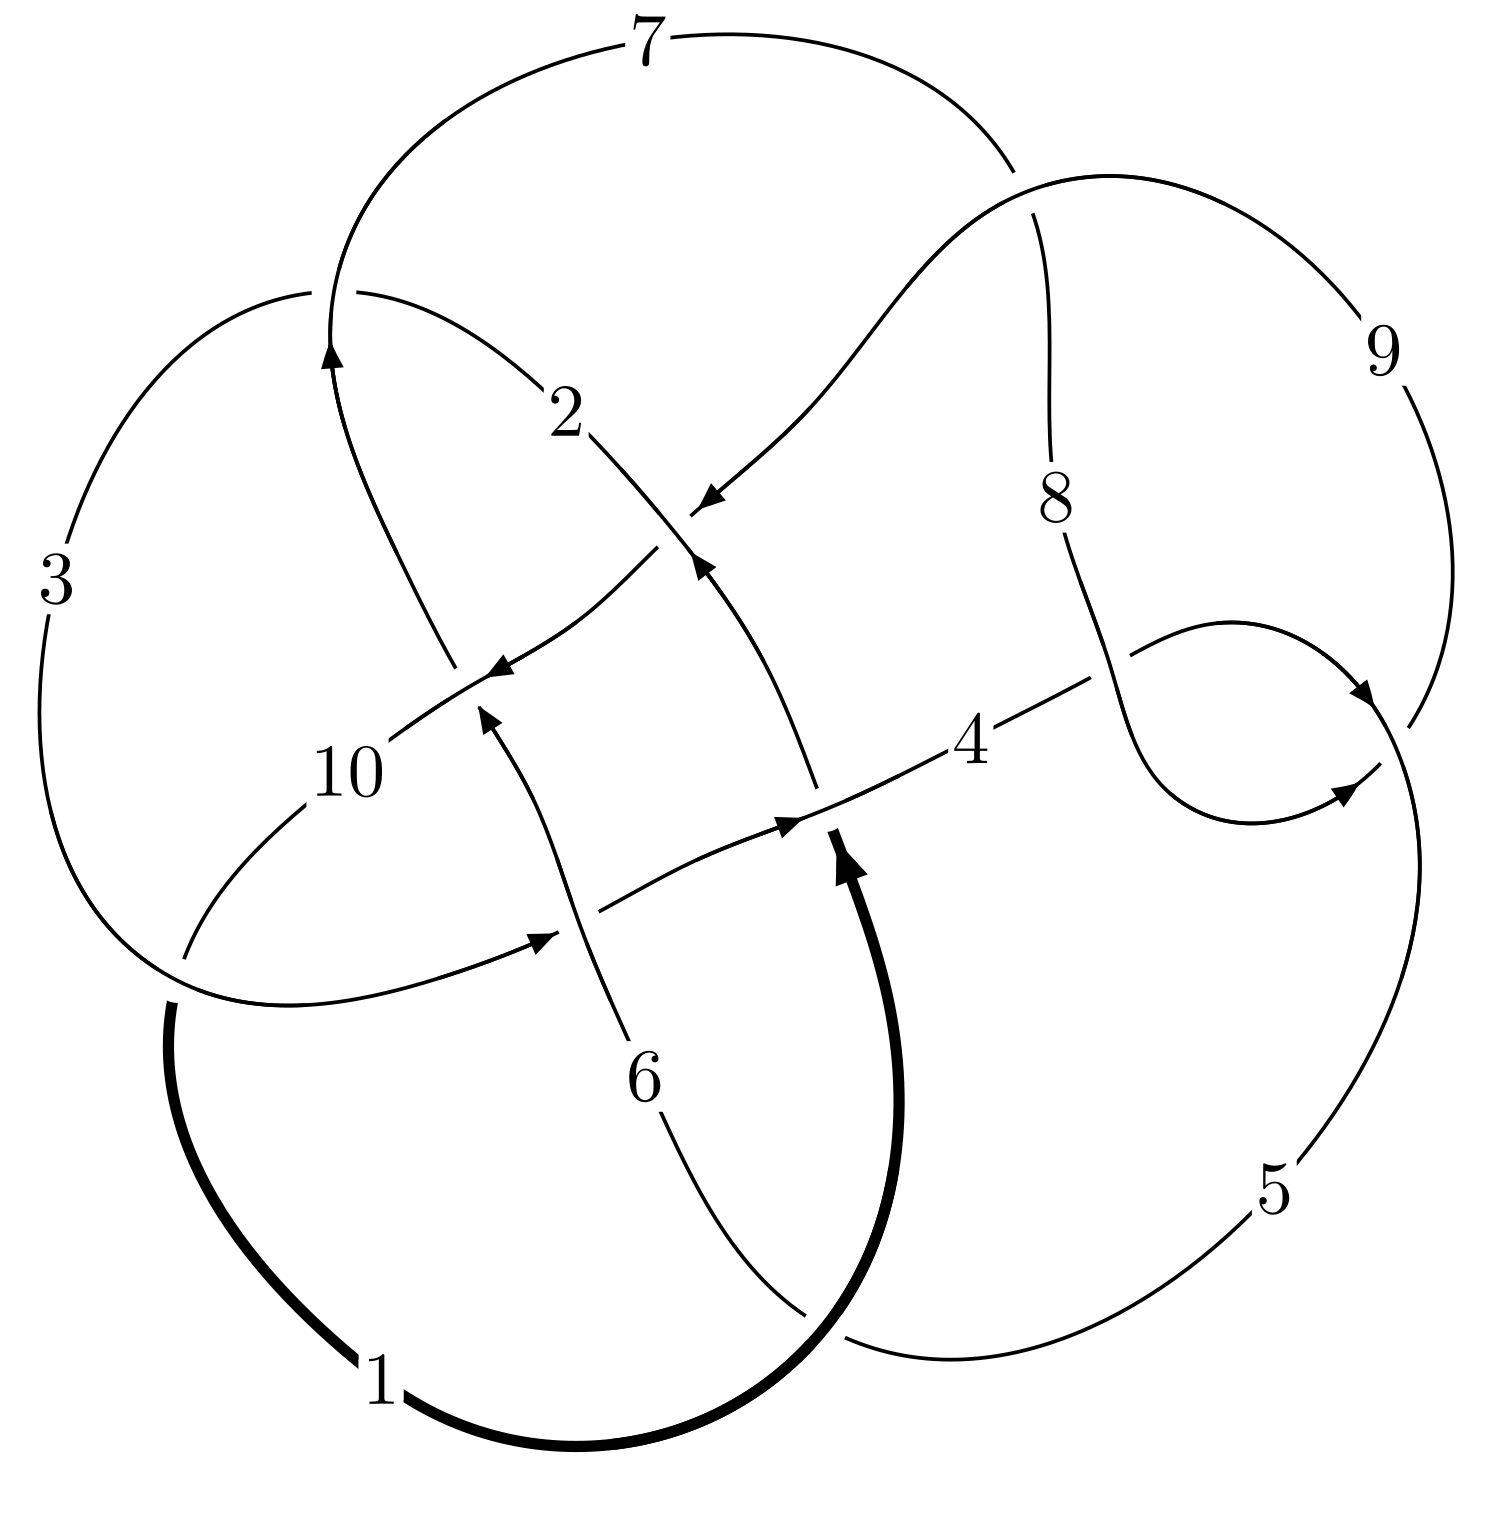
\includegraphics[width=112pt]{../../../GIT/diagram.site/Diagrams/png/197_10_113.png}\\
\ \ \ A knot diagram\footnotemark}&
\allowdisplaybreaks
\textbf{Linearized knot diagam} \\
\cline{2-2}
 &
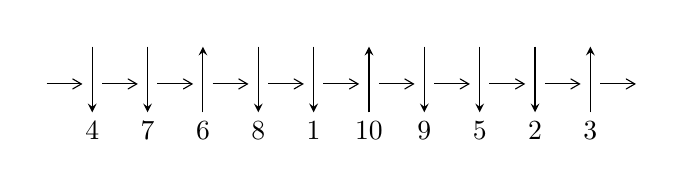
\begin{tikzpicture}[x=20pt, y=17pt]
	% nodes
	\node (C0) at (0, 0) {};
	\node (C1) at (1, 0) {};
	\node (C1U) at (1, +1) {};
	\node (C1D) at (1, -1) {4};

	\node (C2) at (2, 0) {};
	\node (C2U) at (2, +1) {};
	\node (C2D) at (2, -1) {7};

	\node (C3) at (3, 0) {};
	\node (C3U) at (3, +1) {};
	\node (C3D) at (3, -1) {6};

	\node (C4) at (4, 0) {};
	\node (C4U) at (4, +1) {};
	\node (C4D) at (4, -1) {8};

	\node (C5) at (5, 0) {};
	\node (C5U) at (5, +1) {};
	\node (C5D) at (5, -1) {1};

	\node (C6) at (6, 0) {};
	\node (C6U) at (6, +1) {};
	\node (C6D) at (6, -1) {10};

	\node (C7) at (7, 0) {};
	\node (C7U) at (7, +1) {};
	\node (C7D) at (7, -1) {9};

	\node (C8) at (8, 0) {};
	\node (C8U) at (8, +1) {};
	\node (C8D) at (8, -1) {5};

	\node (C9) at (9, 0) {};
	\node (C9U) at (9, +1) {};
	\node (C9D) at (9, -1) {2};

	\node (C10) at (10, 0) {};
	\node (C10U) at (10, +1) {};
	\node (C10D) at (10, -1) {3};
	\node (C11) at (11, 0) {};

	% arrows
	\draw[->,>={angle 60}]
	(C0) edge (C1) (C1) edge (C2) (C2) edge (C3) (C3) edge (C4) (C4) edge (C5) (C5) edge (C6) (C6) edge (C7) (C7) edge (C8) (C8) edge (C9) (C9) edge (C10) (C10) edge (C11) ;	\draw[->,>=stealth]
	(C1U) edge (C1D) (C2U) edge (C2D) (C3D) edge (C3U) (C4U) edge (C4D) (C5U) edge (C5D) (C6D) edge (C6U) (C7U) edge (C7D) (C8U) edge (C8D) (C9U) edge (C9D) (C10D) edge (C10U) ;
	\end{tikzpicture} \\
\hhline{~~} \\& 
\textbf{Solving Sequence} \\ \cline{2-2} 
 &
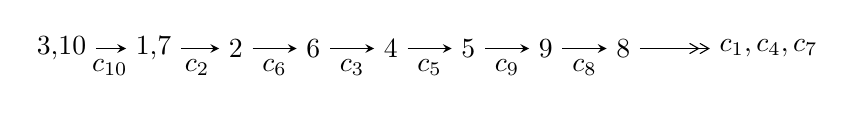
\begin{tikzpicture}[x=28pt, y=7pt]
	% node
	\node (A0) at (-1/8, 0) {3,10};
	\node (A1) at (17/16, 0) {1,7};
	\node (A2) at (17/8, 0) {2};
	\node (A3) at (25/8, 0) {6};
	\node (A4) at (33/8, 0) {4};
	\node (A5) at (41/8, 0) {5};
	\node (A6) at (49/8, 0) {9};
	\node (A7) at (57/8, 0) {8};
	\node (C1) at (1/2, -1) {$c_{10}$};
	\node (C2) at (13/8, -1) {$c_{2}$};
	\node (C3) at (21/8, -1) {$c_{6}$};
	\node (C4) at (29/8, -1) {$c_{3}$};
	\node (C5) at (37/8, -1) {$c_{5}$};
	\node (C6) at (45/8, -1) {$c_{9}$};
	\node (C7) at (53/8, -1) {$c_{8}$};
	\node (A8) at (9, 0) {$c_{1},c_{4},c_{7}$};

	% edge
	\draw[->,>=stealth]	
	(A0) edge (A1) (A1) edge (A2) (A2) edge (A3) (A3) edge (A4) (A4) edge (A5) (A5) edge (A6) (A6) edge (A7) ;
	\draw[->>,>={angle 60}]	
	(A7) edge (A8);
\end{tikzpicture} \\ 

\end{tabular} \\

\footnotetext{
The image of knot diagram is generated by the software ``\textbf{Draw programme}" developed by Andrew Bartholomew(\url{http://www.layer8.co.uk/maths/draw/index.htm\#Running-draw}), where we modified some parts for our purpose(\url{https://github.com/CATsTAILs/LinksPainter}).
}\phantom \\ \newline 
\centering \textbf{Ideals for irreducible components\footnotemark of $X_{\text{par}}$} 
 
\begin{align*}
I^u_{1}&=\langle 
1.09017\times10^{16} u^{25}-1.42680\times10^{17} u^{24}+\cdots+1.22316\times10^{16} b-1.07995\times10^{16},\\
\phantom{I^u_{1}}&\phantom{= \langle  }1.10038\times10^{16} u^{25}-1.55970\times10^{17} u^{24}+\cdots+2.44631\times10^{16} a-3.72028\times10^{16},\;u^{26}-14 u^{25}+\cdots-5 u+2\rangle \\
I^u_{2}&=\langle 
u^{18} a+u^{18}+\cdots-2 a+1,\;2 u^{18} a+3 u^{18}+\cdots-18 a-13,\;u^{19}+9 u^{18}+\cdots- u-2\rangle \\
I^u_{3}&=\langle 
- u^2+b- u-1,\;u^3+3 a- u-1,\;u^4+3 u^3+5 u^2+5 u+3\rangle \\
I^u_{4}&=\langle 
u^2+b+2 u+2,\;- u^2+a- u-2,\;u^3+2 u^2+3 u+1\rangle \\
\\
I^v_{1}&=\langle 
a,\;b+v,\;v^2- v+1\rangle \\
\end{align*}
\raggedright * 5 irreducible components of $\dim_{\mathbb{C}}=0$, with total 73 representations.\\
\footnotetext{All coefficients of polynomials are rational numbers. But the coefficients are sometimes approximated in decimal forms when there is not enough margin.}
\newpage
\renewcommand{\arraystretch}{1}
\centering \section*{I. $I^u_{1}= \langle 1.09\times10^{16} u^{25}-1.43\times10^{17} u^{24}+\cdots+1.22\times10^{16} b-1.08\times10^{16},\;1.10\times10^{16} u^{25}-1.56\times10^{17} u^{24}+\cdots+2.45\times10^{16} a-3.72\times10^{16},\;u^{26}-14 u^{25}+\cdots-5 u+2 \rangle$}
\flushleft \textbf{(i) Arc colorings}\\
\begin{tabular}{m{7pt} m{180pt} m{7pt} m{180pt} }
\flushright $a_{3}=$&$\begin{pmatrix}0\\u\end{pmatrix}$ \\
\flushright $a_{10}=$&$\begin{pmatrix}1\\0\end{pmatrix}$ \\
\flushright $a_{1}=$&$\begin{pmatrix}1\\- u^2\end{pmatrix}$ \\
\flushright $a_{7}=$&$\begin{pmatrix}-0.449813 u^{25}+6.37572 u^{24}+\cdots-2.20872 u+1.52077\\-0.891275 u^{25}+11.6649 u^{24}+\cdots-2.84515 u+0.882924\end{pmatrix}$ \\
\flushright $a_{2}=$&$\begin{pmatrix}0.129701 u^{25}-2.02435 u^{24}+\cdots-4.90429 u+1.76047\\0.0404708 u^{25}-0.734657 u^{24}+\cdots-1.02816 u+0.178460\end{pmatrix}$ \\
\flushright $a_{6}=$&$\begin{pmatrix}0.441462 u^{25}-5.28919 u^{24}+\cdots+0.636436 u+0.637845\\-0.891275 u^{25}+11.6649 u^{24}+\cdots-2.84515 u+0.882924\end{pmatrix}$ \\
\flushright $a_{4}=$&$\begin{pmatrix}0.993712 u^{25}-13.0075 u^{24}+\cdots+1.68701 u-0.405418\\-0.904482 u^{25}+11.7178 u^{24}+\cdots-3.56314 u+1.98742\end{pmatrix}$ \\
\flushright $a_{5}=$&$\begin{pmatrix}0.363122 u^{25}-4.69350 u^{24}+\cdots+1.36473 u-0.261781\\-0.0933259 u^{25}+1.56850 u^{24}+\cdots-0.496488 u-0.119215\end{pmatrix}$ \\
\flushright $a_{9}=$&$\begin{pmatrix}-0.433618 u^{25}+6.06965 u^{24}+\cdots+9.02432 u-0.696343\\0.0726845 u^{25}-0.832738 u^{24}+\cdots+2.33024 u-0.595532\end{pmatrix}$ \\
\flushright $a_{8}=$&$\begin{pmatrix}-0.101086 u^{25}+1.86335 u^{24}+\cdots+7.57533 u-0.827238\\-0.651226 u^{25}+8.60822 u^{24}+\cdots+0.0145807 u+0.0950498\end{pmatrix}$\\&\end{tabular}
\flushleft \textbf{(ii) Obstruction class $= -1$}\\~\\
\flushleft \textbf{(iii) Cusp Shapes $= -\frac{12238612154218315}{12231573450758407} u^{25}+\frac{120808672137987925}{12231573450758407} u^{24}+\cdots+\frac{208460927880809}{12231573450758407} u-\frac{140870794716261400}{12231573450758407}$}\\~\\
\newpage\renewcommand{\arraystretch}{1}
\flushleft \textbf{(iv) u-Polynomials at the component}\newline \\
\begin{tabular}{m{50pt}|m{274pt}}
Crossings & \hspace{64pt}u-Polynomials at each crossing \\
\hline $$\begin{aligned}c_{1},c_{9}\end{aligned}$$&$\begin{aligned}
&u^{26}+4 u^{25}+\cdots-2 u+1
\end{aligned}$\\
\hline $$\begin{aligned}c_{2},c_{5}\end{aligned}$$&$\begin{aligned}
&u^{26}+3 u^{24}+\cdots-2 u+1
\end{aligned}$\\
\hline $$\begin{aligned}c_{3},c_{6}\end{aligned}$$&$\begin{aligned}
&u^{26}+2 u^{25}+\cdots+2 u+1
\end{aligned}$\\
\hline $$\begin{aligned}c_{4},c_{8}\end{aligned}$$&$\begin{aligned}
&u^{26}+6 u^{25}+\cdots+25 u+4
\end{aligned}$\\
\hline $$\begin{aligned}c_{7}\end{aligned}$$&$\begin{aligned}
&u^{26}+10 u^{25}+\cdots+81 u+16
\end{aligned}$\\
\hline $$\begin{aligned}c_{10}\end{aligned}$$&$\begin{aligned}
&u^{26}+14 u^{25}+\cdots+5 u+2
\end{aligned}$\\
\hline
\end{tabular}\\~\\
\newpage\renewcommand{\arraystretch}{1}
\flushleft \textbf{(v) Riley Polynomials at the component}\newline \\
\begin{tabular}{m{50pt}|m{274pt}}
Crossings & \hspace{64pt}Riley Polynomials at each crossing \\
\hline $$\begin{aligned}c_{1},c_{9}\end{aligned}$$&$\begin{aligned}
&y^{26}-10 y^{25}+\cdots-18 y+1
\end{aligned}$\\
\hline $$\begin{aligned}c_{2},c_{5}\end{aligned}$$&$\begin{aligned}
&y^{26}+6 y^{25}+\cdots+6 y+1
\end{aligned}$\\
\hline $$\begin{aligned}c_{3},c_{6}\end{aligned}$$&$\begin{aligned}
&y^{26}+14 y^{25}+\cdots+30 y+1
\end{aligned}$\\
\hline $$\begin{aligned}c_{4},c_{8}\end{aligned}$$&$\begin{aligned}
&y^{26}-10 y^{25}+\cdots-81 y+16
\end{aligned}$\\
\hline $$\begin{aligned}c_{7}\end{aligned}$$&$\begin{aligned}
&y^{26}+10 y^{25}+\cdots+9439 y+256
\end{aligned}$\\
\hline $$\begin{aligned}c_{10}\end{aligned}$$&$\begin{aligned}
&y^{26}+8 y^{24}+\cdots-21 y+4
\end{aligned}$\\
\hline
\end{tabular}\\~\\
\newpage\flushleft \textbf{(vi) Complex Volumes and Cusp Shapes}
$$\begin{array}{c|c|c}  
\text{Solutions to }I^u_{1}& \I (\text{vol} + \sqrt{-1}CS) & \text{Cusp shape}\\
 \hline 
\begin{aligned}
u &= \phantom{-}1.056680 + 0.510753 I \\
a &= -0.215461 + 0.700629 I \\
b &= \phantom{-}1.09337 + 1.26772 I\end{aligned}
 & \phantom{-}1.49747 + 5.09068 I & -3.0367 - 14.8892 I \\ \hline\begin{aligned}
u &= \phantom{-}1.056680 - 0.510753 I \\
a &= -0.215461 - 0.700629 I \\
b &= \phantom{-}1.09337 - 1.26772 I\end{aligned}
 & \phantom{-}1.49747 - 5.09068 I & -3.0367 + 14.8892 I \\ \hline\begin{aligned}
u &= -1.197700 + 0.220817 I \\
a &= \phantom{-}0.079663 - 0.840370 I \\
b &= \phantom{-}0.005740 - 0.465412 I\end{aligned}
 & \phantom{-}2.92221 - 2.66541 I & \phantom{-}1.40924 + 2.72285 I \\ \hline\begin{aligned}
u &= -1.197700 - 0.220817 I \\
a &= \phantom{-}0.079663 + 0.840370 I \\
b &= \phantom{-}0.005740 + 0.465412 I\end{aligned}
 & \phantom{-}2.92221 + 2.66541 I & \phantom{-}1.40924 - 2.72285 I \\ \hline\begin{aligned}
u &= \phantom{-}1.306830 + 0.079067 I \\
a &= -0.107470 + 0.279551 I \\
b &= -0.215760 + 1.218550 I\end{aligned}
 & -0.13330 + 3.14853 I & -10.05225 - 4.78603 I \\ \hline\begin{aligned}
u &= \phantom{-}1.306830 - 0.079067 I \\
a &= -0.107470 - 0.279551 I \\
b &= -0.215760 - 1.218550 I\end{aligned}
 & -0.13330 - 3.14853 I & -10.05225 + 4.78603 I \\ \hline\begin{aligned}
u &= \phantom{-}0.493624 + 0.435869 I \\
a &= \phantom{-}0.905680 - 0.839887 I \\
b &= -0.941763 - 0.771472 I\end{aligned}
 & -2.18699 - 0.53885 I & -10.45014 + 2.98932 I \\ \hline\begin{aligned}
u &= \phantom{-}0.493624 - 0.435869 I \\
a &= \phantom{-}0.905680 + 0.839887 I \\
b &= -0.941763 + 0.771472 I\end{aligned}
 & -2.18699 + 0.53885 I & -10.45014 - 2.98932 I \\ \hline\begin{aligned}
u &= \phantom{-}1.022930 + 0.871070 I \\
a &= \phantom{-}0.149244 - 0.992194 I \\
b &= -0.98451 - 1.19337 I\end{aligned}
 & -4.53791 + 8.53907 I & -8.63796 - 7.50515 I \\ \hline\begin{aligned}
u &= \phantom{-}1.022930 - 0.871070 I \\
a &= \phantom{-}0.149244 + 0.992194 I \\
b &= -0.98451 + 1.19337 I\end{aligned}
 & -4.53791 - 8.53907 I & -8.63796 + 7.50515 I\\
 \hline 
 \end{array}$$\newpage$$\begin{array}{c|c|c}  
\text{Solutions to }I^u_{1}& \I (\text{vol} + \sqrt{-1}CS) & \text{Cusp shape}\\
 \hline 
\begin{aligned}
u &= \phantom{-}0.129304 + 0.643314 I \\
a &= \phantom{-}0.984267 - 0.517979 I \\
b &= -0.031311 - 0.673436 I\end{aligned}
 & -0.924615 - 1.060120 I & -5.32469 + 4.59251 I \\ \hline\begin{aligned}
u &= \phantom{-}0.129304 - 0.643314 I \\
a &= \phantom{-}0.984267 + 0.517979 I \\
b &= -0.031311 + 0.673436 I\end{aligned}
 & -0.924615 + 1.060120 I & -5.32469 - 4.59251 I \\ \hline\begin{aligned}
u &= \phantom{-}0.967641 + 1.016650 I \\
a &= -0.486502 + 0.264040 I \\
b &= -0.211831 + 0.733834 I\end{aligned}
 & -4.93342 - 1.67636 I & -14.6461 + 4.2929 I \\ \hline\begin{aligned}
u &= \phantom{-}0.967641 - 1.016650 I \\
a &= -0.486502 - 0.264040 I \\
b &= -0.211831 - 0.733834 I\end{aligned}
 & -4.93342 + 1.67636 I & -14.6461 - 4.2929 I \\ \hline\begin{aligned}
u &= \phantom{-}1.26531 + 0.92939 I \\
a &= \phantom{-}0.020000 + 0.955891 I \\
b &= \phantom{-}0.97670 + 1.20748 I\end{aligned}
 & \phantom{-}2.62082 + 10.45440 I & -1.93774 - 5.95159 I \\ \hline\begin{aligned}
u &= \phantom{-}1.26531 - 0.92939 I \\
a &= \phantom{-}0.020000 - 0.955891 I \\
b &= \phantom{-}0.97670 - 1.20748 I\end{aligned}
 & \phantom{-}2.62082 - 10.45440 I & -1.93774 + 5.95159 I \\ \hline\begin{aligned}
u &= -0.014473 + 0.410285 I \\
a &= -2.05321 + 1.74511 I \\
b &= \phantom{-}0.284111 + 0.970184 I\end{aligned}
 & -1.92544 + 2.11547 I & -8.52748 - 4.72090 I \\ \hline\begin{aligned}
u &= -0.014473 - 0.410285 I \\
a &= -2.05321 - 1.74511 I \\
b &= \phantom{-}0.284111 - 0.970184 I\end{aligned}
 & -1.92544 - 2.11547 I & -8.52748 + 4.72090 I \\ \hline\begin{aligned}
u &= \phantom{-}0.34430 + 1.56008 I \\
a &= \phantom{-}0.493219 - 0.417449 I \\
b &= \phantom{-}0.152881 - 0.590554 I\end{aligned}
 & \phantom{-}0.16560 - 2.24390 I & -7.60792 + 3.01225 I \\ \hline\begin{aligned}
u &= \phantom{-}0.34430 - 1.56008 I \\
a &= \phantom{-}0.493219 + 0.417449 I \\
b &= \phantom{-}0.152881 + 0.590554 I\end{aligned}
 & \phantom{-}0.16560 + 2.24390 I & -7.60792 - 3.01225 I\\
 \hline 
 \end{array}$$\newpage$$\begin{array}{c|c|c}  
\text{Solutions to }I^u_{1}& \I (\text{vol} + \sqrt{-1}CS) & \text{Cusp shape}\\
 \hline 
\begin{aligned}
u &= \phantom{-}1.26295 + 1.01918 I \\
a &= -0.042904 - 1.006760 I \\
b &= -0.97925 - 1.20625 I\end{aligned}
 & \phantom{-}0.9109 + 16.4735 I & -4.00000 - 9.70500 I \\ \hline\begin{aligned}
u &= \phantom{-}1.26295 - 1.01918 I \\
a &= -0.042904 + 1.006760 I \\
b &= -0.97925 + 1.20625 I\end{aligned}
 & \phantom{-}0.9109 - 16.4735 I & -4.00000 + 9.70500 I \\ \hline\begin{aligned}
u &= -0.281192 + 0.094635 I \\
a &= -1.01688 + 4.90932 I \\
b &= \phantom{-}0.054013 + 1.156590 I\end{aligned}
 & -1.56544 - 2.09555 I & -7.86102 + 3.20965 I \\ \hline\begin{aligned}
u &= -0.281192 - 0.094635 I \\
a &= -1.01688 - 4.90932 I \\
b &= \phantom{-}0.054013 - 1.156590 I\end{aligned}
 & -1.56544 + 2.09555 I & -7.86102 - 3.20965 I \\ \hline\begin{aligned}
u &= \phantom{-}0.64380 + 1.75632 I \\
a &= -0.459645 + 0.377201 I \\
b &= -0.202381 + 0.586735 I\end{aligned}
 & -0.95700 - 7.52275 I & \phantom{-0.000000 } 0 \\ \hline\begin{aligned}
u &= \phantom{-}0.64380 - 1.75632 I \\
a &= -0.459645 - 0.377201 I \\
b &= -0.202381 - 0.586735 I\end{aligned}
 & -0.95700 + 7.52275 I & \phantom{-0.000000 } 0\\
 \hline 
 \end{array}$$\newpage\newpage\renewcommand{\arraystretch}{1}
\centering \section*{II. $I^u_{2}= \langle u^{18} a+u^{18}+\cdots-2 a+1,\;2 u^{18} a+3 u^{18}+\cdots-18 a-13,\;u^{19}+9 u^{18}+\cdots- u-2 \rangle$}
\flushleft \textbf{(i) Arc colorings}\\
\begin{tabular}{m{7pt} m{180pt} m{7pt} m{180pt} }
\flushright $a_{3}=$&$\begin{pmatrix}0\\u\end{pmatrix}$ \\
\flushright $a_{10}=$&$\begin{pmatrix}1\\0\end{pmatrix}$ \\
\flushright $a_{1}=$&$\begin{pmatrix}1\\- u^2\end{pmatrix}$ \\
\flushright $a_{7}=$&$\begin{pmatrix}a\\- u^{18} a- u^{18}+\cdots+2 a-1\end{pmatrix}$ \\
\flushright $a_{2}=$&$\begin{pmatrix}u^{18} a+\frac{1}{2} u^{18}+\cdots- a-\frac{3}{2}\\u^{18}+8 u^{17}+\cdots-2 a-1\end{pmatrix}$ \\
\flushright $a_{6}=$&$\begin{pmatrix}u^{18} a+u^{18}+\cdots- a+1\\- u^{18} a- u^{18}+\cdots+2 a-1\end{pmatrix}$ \\
\flushright $a_{4}=$&$\begin{pmatrix}u^{18} a-\frac{1}{2} u^{18}+\cdots+a+\frac{1}{2}\\-1\end{pmatrix}$ \\
\flushright $a_{5}=$&$\begin{pmatrix}u^{18} a+8 u^{17} a+\cdots- a+2\\- u^{18} a-2 u^{18}+\cdots+2 a+1\end{pmatrix}$ \\
\flushright $a_{9}=$&$\begin{pmatrix}-\frac{1}{2} u^{18}-\frac{7}{2} u^{17}+\cdots- a+\frac{1}{2}\\- u^{18} a+u^{18}+\cdots+u-3\end{pmatrix}$ \\
\flushright $a_{8}=$&$\begin{pmatrix}u^{17} a-\frac{1}{2} u^{18}+\cdots+2 a+\frac{1}{2}\\- u^{17}-8 u^{16}+\cdots-3 u-2\end{pmatrix}$\\&\end{tabular}
\flushleft \textbf{(ii) Obstruction class $= -1$}\\~\\
\flushleft \textbf{(iii) Cusp Shapes $= -5 u^{18}-43 u^{17}-177 u^{16}-432 u^{15}-640 u^{14}-457 u^{13}+209 u^{12}+824 u^{11}+687 u^{10}-101 u^9-627 u^8-368 u^7+164 u^6+274 u^5+34 u^4-104 u^3-41 u^2+25 u+9$}\\~\\
\newpage\renewcommand{\arraystretch}{1}
\flushleft \textbf{(iv) u-Polynomials at the component}\newline \\
\begin{tabular}{m{50pt}|m{274pt}}
Crossings & \hspace{64pt}u-Polynomials at each crossing \\
\hline $$\begin{aligned}c_{1},c_{9}\end{aligned}$$&$\begin{aligned}
&u^{38}-3 u^{37}+\cdots+10 u-1
\end{aligned}$\\
\hline $$\begin{aligned}c_{2},c_{5}\end{aligned}$$&$\begin{aligned}
&u^{38}+2 u^{37}+\cdots+109 u+11
\end{aligned}$\\
\hline $$\begin{aligned}c_{3},c_{6}\end{aligned}$$&$\begin{aligned}
&u^{38}+4 u^{37}+\cdots+7 u+1
\end{aligned}$\\
\hline $$\begin{aligned}c_{4},c_{8}\end{aligned}$$&$\begin{aligned}
&(u^{19}-2 u^{18}+\cdots-4 u+1)^{2}
\end{aligned}$\\
\hline $$\begin{aligned}c_{7}\end{aligned}$$&$\begin{aligned}
&(u^{19}+8 u^{18}+\cdots+4 u+1)^{2}
\end{aligned}$\\
\hline $$\begin{aligned}c_{10}\end{aligned}$$&$\begin{aligned}
&(u^{19}-9 u^{18}+\cdots- u+2)^{2}
\end{aligned}$\\
\hline
\end{tabular}\\~\\
\newpage\renewcommand{\arraystretch}{1}
\flushleft \textbf{(v) Riley Polynomials at the component}\newline \\
\begin{tabular}{m{50pt}|m{274pt}}
Crossings & \hspace{64pt}Riley Polynomials at each crossing \\
\hline $$\begin{aligned}c_{1},c_{9}\end{aligned}$$&$\begin{aligned}
&y^{38}+13 y^{37}+\cdots+2 y+1
\end{aligned}$\\
\hline $$\begin{aligned}c_{2},c_{5}\end{aligned}$$&$\begin{aligned}
&y^{38}+4 y^{37}+\cdots-13311 y+121
\end{aligned}$\\
\hline $$\begin{aligned}c_{3},c_{6}\end{aligned}$$&$\begin{aligned}
&y^{38}-8 y^{37}+\cdots+5 y+1
\end{aligned}$\\
\hline $$\begin{aligned}c_{4},c_{8}\end{aligned}$$&$\begin{aligned}
&(y^{19}-8 y^{18}+\cdots+4 y-1)^{2}
\end{aligned}$\\
\hline $$\begin{aligned}c_{7}\end{aligned}$$&$\begin{aligned}
&(y^{19}+8 y^{18}+\cdots-16 y-1)^{2}
\end{aligned}$\\
\hline $$\begin{aligned}c_{10}\end{aligned}$$&$\begin{aligned}
&(y^{19}-3 y^{18}+\cdots+37 y-4)^{2}
\end{aligned}$\\
\hline
\end{tabular}\\~\\
\newpage\flushleft \textbf{(vi) Complex Volumes and Cusp Shapes}
$$\begin{array}{c|c|c}  
\text{Solutions to }I^u_{2}& \I (\text{vol} + \sqrt{-1}CS) & \text{Cusp shape}\\
 \hline 
\begin{aligned}
u &= -0.488744 + 1.038280 I \\
a &= -0.478820 + 0.914222 I \\
b &= -1.13156 + 1.02165 I\end{aligned}
 & -1.59095 - 7.59815 I & -9.53397 + 8.95368 I \\ \hline\begin{aligned}
u &= -0.488744 + 1.038280 I \\
a &= -1.01797 - 1.24322 I \\
b &= \phantom{-}0.207487 - 0.730234 I\end{aligned}
 & -1.59095 - 7.59815 I & -9.53397 + 8.95368 I \\ \hline\begin{aligned}
u &= -0.488744 - 1.038280 I \\
a &= -0.478820 - 0.914222 I \\
b &= -1.13156 - 1.02165 I\end{aligned}
 & -1.59095 + 7.59815 I & -9.53397 - 8.95368 I \\ \hline\begin{aligned}
u &= -0.488744 - 1.038280 I \\
a &= -1.01797 + 1.24322 I \\
b &= \phantom{-}0.207487 + 0.730234 I\end{aligned}
 & -1.59095 + 7.59815 I & -9.53397 - 8.95368 I \\ \hline\begin{aligned}
u &= -0.752606 + 0.874521 I \\
a &= \phantom{-}0.794589 + 0.607095 I \\
b &= -0.361281 + 0.577577 I\end{aligned}
 & \phantom{-}0.10793 - 3.14909 I & -5.58222 + 3.79428 I \\ \hline\begin{aligned}
u &= -0.752606 + 0.874521 I \\
a &= \phantom{-}0.312041 - 0.899421 I \\
b &= \phantom{-}0.895728 - 0.988619 I\end{aligned}
 & \phantom{-}0.10793 - 3.14909 I & -5.58222 + 3.79428 I \\ \hline\begin{aligned}
u &= -0.752606 - 0.874521 I \\
a &= \phantom{-}0.794589 - 0.607095 I \\
b &= -0.361281 - 0.577577 I\end{aligned}
 & \phantom{-}0.10793 + 3.14909 I & -5.58222 - 3.79428 I \\ \hline\begin{aligned}
u &= -0.752606 - 0.874521 I \\
a &= \phantom{-}0.312041 + 0.899421 I \\
b &= \phantom{-}0.895728 + 0.988619 I\end{aligned}
 & \phantom{-}0.10793 + 3.14909 I & -5.58222 - 3.79428 I \\ \hline\begin{aligned}
u &= -1.211130 + 0.137559 I \\
a &= \phantom{-}0.091441 - 0.907433 I \\
b &= \phantom{-}0.287046 - 0.731500 I\end{aligned}
 & \phantom{-}2.95026 - 2.66622 I & \phantom{-}1.58619 + 3.20879 I \\ \hline\begin{aligned}
u &= -1.211130 + 0.137559 I \\
a &= \phantom{-}0.040607 - 0.755883 I \\
b &= -0.261106 - 0.186172 I\end{aligned}
 & \phantom{-}2.95026 - 2.66622 I & \phantom{-}1.58619 + 3.20879 I\\
 \hline 
 \end{array}$$\newpage$$\begin{array}{c|c|c}  
\text{Solutions to }I^u_{2}& \I (\text{vol} + \sqrt{-1}CS) & \text{Cusp shape}\\
 \hline 
\begin{aligned}
u &= -1.211130 - 0.137559 I \\
a &= \phantom{-}0.091441 + 0.907433 I \\
b &= \phantom{-}0.287046 + 0.731500 I\end{aligned}
 & \phantom{-}2.95026 + 2.66622 I & \phantom{-}1.58619 - 3.20879 I \\ \hline\begin{aligned}
u &= -1.211130 - 0.137559 I \\
a &= \phantom{-}0.040607 + 0.755883 I \\
b &= -0.261106 + 0.186172 I\end{aligned}
 & \phantom{-}2.95026 + 2.66622 I & \phantom{-}1.58619 - 3.20879 I \\ \hline\begin{aligned}
u &= \phantom{-}0.687103 + 0.235969 I \\
a &= -0.068144 + 1.145470 I \\
b &= -1.44986 + 0.74441 I\end{aligned}
 & \phantom{-}2.42247 + 8.22022 I & -0.13214 - 8.57000 I \\ \hline\begin{aligned}
u &= \phantom{-}0.687103 + 0.235969 I \\
a &= \phantom{-}0.69993 - 2.21894 I \\
b &= -0.854742 - 0.601611 I\end{aligned}
 & \phantom{-}2.42247 + 8.22022 I & -0.13214 - 8.57000 I \\ \hline\begin{aligned}
u &= \phantom{-}0.687103 - 0.235969 I \\
a &= -0.068144 - 1.145470 I \\
b &= -1.44986 - 0.74441 I\end{aligned}
 & \phantom{-}2.42247 - 8.22022 I & -0.13214 + 8.57000 I \\ \hline\begin{aligned}
u &= \phantom{-}0.687103 - 0.235969 I \\
a &= \phantom{-}0.69993 + 2.21894 I \\
b &= -0.854742 + 0.601611 I\end{aligned}
 & \phantom{-}2.42247 - 8.22022 I & -0.13214 + 8.57000 I \\ \hline\begin{aligned}
u &= \phantom{-}0.689008 + 0.139635 I \\
a &= -0.128846 - 1.148580 I \\
b &= \phantom{-}1.37561 - 0.64670 I\end{aligned}
 & \phantom{-}4.26470 + 2.32942 I & \phantom{-}3.40004 - 3.00608 I \\ \hline\begin{aligned}
u &= \phantom{-}0.689008 + 0.139635 I \\
a &= -0.76853 + 1.84609 I \\
b &= \phantom{-}0.966499 + 0.555876 I\end{aligned}
 & \phantom{-}4.26470 + 2.32942 I & \phantom{-}3.40004 - 3.00608 I \\ \hline\begin{aligned}
u &= \phantom{-}0.689008 - 0.139635 I \\
a &= -0.128846 + 1.148580 I \\
b &= \phantom{-}1.37561 + 0.64670 I\end{aligned}
 & \phantom{-}4.26470 - 2.32942 I & \phantom{-}3.40004 + 3.00608 I \\ \hline\begin{aligned}
u &= \phantom{-}0.689008 - 0.139635 I \\
a &= -0.76853 - 1.84609 I \\
b &= \phantom{-}0.966499 - 0.555876 I\end{aligned}
 & \phantom{-}4.26470 - 2.32942 I & \phantom{-}3.40004 + 3.00608 I\\
 \hline 
 \end{array}$$\newpage$$\begin{array}{c|c|c}  
\text{Solutions to }I^u_{2}& \I (\text{vol} + \sqrt{-1}CS) & \text{Cusp shape}\\
 \hline 
\begin{aligned}
u &= -0.378245 + 0.567353 I \\
a &= -0.400712 + 1.127850 I \\
b &= -1.02428 + 1.44155 I\end{aligned}
 & -3.84277 - 0.76131 I & -13.4982 + 7.0538 I \\ \hline\begin{aligned}
u &= -0.378245 + 0.567353 I \\
a &= -2.53438 - 0.54959 I \\
b &= \phantom{-}0.057884 - 0.472439 I\end{aligned}
 & -3.84277 - 0.76131 I & -13.4982 + 7.0538 I \\ \hline\begin{aligned}
u &= -0.378245 - 0.567353 I \\
a &= -0.400712 - 1.127850 I \\
b &= -1.02428 - 1.44155 I\end{aligned}
 & -3.84277 + 0.76131 I & -13.4982 - 7.0538 I \\ \hline\begin{aligned}
u &= -0.378245 - 0.567353 I \\
a &= -2.53438 + 0.54959 I \\
b &= \phantom{-}0.057884 + 0.472439 I\end{aligned}
 & -3.84277 + 0.76131 I & -13.4982 - 7.0538 I \\ \hline\begin{aligned}
u &= -0.865146 + 1.042810 I \\
a &= \phantom{-}0.422088 + 0.852186 I \\
b &= -0.475702 + 0.708695 I\end{aligned}
 & \phantom{-}0.09217 - 3.26203 I & -7.82857 + 4.58696 I \\ \hline\begin{aligned}
u &= -0.865146 + 1.042810 I \\
a &= \phantom{-}0.299650 - 0.748328 I \\
b &= \phantom{-}0.926354 - 0.812087 I\end{aligned}
 & \phantom{-}0.09217 - 3.26203 I & -7.82857 + 4.58696 I \\ \hline\begin{aligned}
u &= -0.865146 - 1.042810 I \\
a &= \phantom{-}0.422088 - 0.852186 I \\
b &= -0.475702 - 0.708695 I\end{aligned}
 & \phantom{-}0.09217 + 3.26203 I & -7.82857 - 4.58696 I \\ \hline\begin{aligned}
u &= -0.865146 - 1.042810 I \\
a &= \phantom{-}0.299650 + 0.748328 I \\
b &= \phantom{-}0.926354 + 0.812087 I\end{aligned}
 & \phantom{-}0.09217 + 3.26203 I & -7.82857 - 4.58696 I \\ \hline\begin{aligned}
u &= \phantom{-}0.494703\phantom{ +0.000000I} \\
a &= \phantom{-}0.176592\phantom{ +0.000000I} \\
b &= -1.65217\phantom{ +0.000000I}\end{aligned}
 & -2.37666\phantom{ +0.000000I} & \phantom{-}7.11410\phantom{ +0.000000I} \\ \hline\begin{aligned}
u &= \phantom{-}0.494703\phantom{ +0.000000I} \\
a &= \phantom{-}2.43502\phantom{ +0.000000I} \\
b &= -0.904693\phantom{ +0.000000I}\end{aligned}
 & -2.37666\phantom{ +0.000000I} & \phantom{-}7.11410\phantom{ +0.000000I}\\
 \hline 
 \end{array}$$\newpage$$\begin{array}{c|c|c}  
\text{Solutions to }I^u_{2}& \I (\text{vol} + \sqrt{-1}CS) & \text{Cusp shape}\\
 \hline 
\begin{aligned}
u &= -1.23842 + 1.01885 I \\
a &= \phantom{-}0.079408 - 1.045930 I \\
b &= \phantom{-}0.651625 - 0.880608 I\end{aligned}
 & \phantom{-}2.68628 - 1.90197 I & \phantom{-}1.62421 + 1.37993 I \\ \hline\begin{aligned}
u &= -1.23842 + 1.01885 I \\
a &= -0.214414 + 0.212371 I \\
b &= -0.877077 + 0.378271 I\end{aligned}
 & \phantom{-}2.68628 - 1.90197 I & \phantom{-}1.62421 + 1.37993 I \\ \hline\begin{aligned}
u &= -1.23842 - 1.01885 I \\
a &= \phantom{-}0.079408 + 1.045930 I \\
b &= \phantom{-}0.651625 + 0.880608 I\end{aligned}
 & \phantom{-}2.68628 + 1.90197 I & \phantom{-}1.62421 - 1.37993 I \\ \hline\begin{aligned}
u &= -1.23842 - 1.01885 I \\
a &= -0.214414 - 0.212371 I \\
b &= -0.877077 - 0.378271 I\end{aligned}
 & \phantom{-}2.68628 + 1.90197 I & \phantom{-}1.62421 - 1.37993 I \\ \hline\begin{aligned}
u &= -1.18917 + 1.13858 I \\
a &= -0.003038 + 1.092820 I \\
b &= -0.617784 + 0.888572 I\end{aligned}
 & \phantom{-}2.32292 - 6.77576 I & -0.09240 + 8.89089 I \\ \hline\begin{aligned}
u &= -1.18917 + 1.13858 I \\
a &= \phantom{-}0.319294 - 0.326713 I \\
b &= \phantom{-}0.963591 - 0.457047 I\end{aligned}
 & \phantom{-}2.32292 - 6.77576 I & -0.09240 + 8.89089 I \\ \hline\begin{aligned}
u &= -1.18917 - 1.13858 I \\
a &= -0.003038 - 1.092820 I \\
b &= -0.617784 - 0.888572 I\end{aligned}
 & \phantom{-}2.32292 + 6.77576 I & -0.09240 - 8.89089 I \\ \hline\begin{aligned}
u &= -1.18917 - 1.13858 I \\
a &= \phantom{-}0.319294 + 0.326713 I \\
b &= \phantom{-}0.963591 + 0.457047 I\end{aligned}
 & \phantom{-}2.32292 + 6.77576 I & -0.09240 - 8.89089 I\\
 \hline 
 \end{array}$$\newpage\newpage\renewcommand{\arraystretch}{1}
\centering \section*{III. $I^u_{3}= \langle - u^2+b- u-1,\;u^3+3 a- u-1,\;u^4+3 u^3+5 u^2+5 u+3 \rangle$}
\flushleft \textbf{(i) Arc colorings}\\
\begin{tabular}{m{7pt} m{180pt} m{7pt} m{180pt} }
\flushright $a_{3}=$&$\begin{pmatrix}0\\u\end{pmatrix}$ \\
\flushright $a_{10}=$&$\begin{pmatrix}1\\0\end{pmatrix}$ \\
\flushright $a_{1}=$&$\begin{pmatrix}1\\- u^2\end{pmatrix}$ \\
\flushright $a_{7}=$&$\begin{pmatrix}-\frac{1}{3} u^3+\frac{1}{3} u+\frac{1}{3}\\u^2+u+1\end{pmatrix}$ \\
\flushright $a_{2}=$&$\begin{pmatrix}-\frac{1}{3} u^3- u^2-\frac{5}{3} u-\frac{2}{3}\\u+1\end{pmatrix}$ \\
\flushright $a_{6}=$&$\begin{pmatrix}-\frac{1}{3} u^3- u^2-\frac{2}{3} u-\frac{2}{3}\\u^2+u+1\end{pmatrix}$ \\
\flushright $a_{4}=$&$\begin{pmatrix}\frac{2}{3} u^3+u^2+\frac{4}{3} u+\frac{1}{3}\\- u^3-2 u^2-2 u-2\end{pmatrix}$ \\
\flushright $a_{5}=$&$\begin{pmatrix}\frac{2}{3} u^3+u^2+\frac{4}{3} u+\frac{1}{3}\\- u-2\end{pmatrix}$ \\
\flushright $a_{9}=$&$\begin{pmatrix}\frac{1}{3} u^3+u^2+\frac{2}{3} u+\frac{2}{3}\\- u^2-2 u-1\end{pmatrix}$ \\
\flushright $a_{8}=$&$\begin{pmatrix}0\\- u^3-2 u^2-2 u\end{pmatrix}$\\&\end{tabular}
\flushleft \textbf{(ii) Obstruction class $= 1$}\\~\\
\flushleft \textbf{(iii) Cusp Shapes $= 3 u^3+8 u^2+16 u+9$}\\~\\
\newpage\renewcommand{\arraystretch}{1}
\flushleft \textbf{(iv) u-Polynomials at the component}\newline \\
\begin{tabular}{m{50pt}|m{274pt}}
Crossings & \hspace{64pt}u-Polynomials at each crossing \\
\hline $$\begin{aligned}c_{1},c_{7},c_{9}\end{aligned}$$&$\begin{aligned}
&u^4- u^3+2 u^2+1
\end{aligned}$\\
\hline $$\begin{aligned}c_{2},c_{5},c_{8}\end{aligned}$$&$\begin{aligned}
&u^4- u^3+1
\end{aligned}$\\
\hline $$\begin{aligned}c_{3},c_{6}\end{aligned}$$&$\begin{aligned}
&u^4- u+1
\end{aligned}$\\
\hline $$\begin{aligned}c_{4}\end{aligned}$$&$\begin{aligned}
&u^4+u^3+1
\end{aligned}$\\
\hline $$\begin{aligned}c_{10}\end{aligned}$$&$\begin{aligned}
&u^4+3 u^3+5 u^2+5 u+3
\end{aligned}$\\
\hline
\end{tabular}\\~\\
\newpage\renewcommand{\arraystretch}{1}
\flushleft \textbf{(v) Riley Polynomials at the component}\newline \\
\begin{tabular}{m{50pt}|m{274pt}}
Crossings & \hspace{64pt}Riley Polynomials at each crossing \\
\hline $$\begin{aligned}c_{1},c_{7},c_{9}\end{aligned}$$&$\begin{aligned}
&y^4+3 y^3+6 y^2+4 y+1
\end{aligned}$\\
\hline $$\begin{aligned}c_{2},c_{4},c_{5}\\c_{8}\end{aligned}$$&$\begin{aligned}
&y^4- y^3+2 y^2+1
\end{aligned}$\\
\hline $$\begin{aligned}c_{3},c_{6}\end{aligned}$$&$\begin{aligned}
&y^4+2 y^2- y+1
\end{aligned}$\\
\hline $$\begin{aligned}c_{10}\end{aligned}$$&$\begin{aligned}
&y^4+y^3+y^2+5 y+9
\end{aligned}$\\
\hline
\end{tabular}\\~\\
\newpage\flushleft \textbf{(vi) Complex Volumes and Cusp Shapes}
$$\begin{array}{c|c|c}  
\text{Solutions to }I^u_{3}& \I (\text{vol} + \sqrt{-1}CS) & \text{Cusp shape}\\
 \hline 
\begin{aligned}
u &= -0.324902 + 1.227920 I \\
a &= -0.253420 + 0.896839 I \\
b &= -0.727136 + 0.430014 I\end{aligned}
 & \phantom{-}0.20545 - 7.54387 I & -3.11022 + 8.87572 I \\ \hline\begin{aligned}
u &= -0.324902 - 1.227920 I \\
a &= -0.253420 - 0.896839 I \\
b &= -0.727136 - 0.430014 I\end{aligned}
 & \phantom{-}0.20545 + 7.54387 I & -3.11022 - 8.87572 I \\ \hline\begin{aligned}
u &= -1.175100 + 0.691825 I \\
a &= -0.079913 - 0.614328 I \\
b &= \phantom{-}0.727136 - 0.934099 I\end{aligned}
 & \phantom{-}1.43949 - 4.22398 I & -2.38978 + 5.66623 I \\ \hline\begin{aligned}
u &= -1.175100 - 0.691825 I \\
a &= -0.079913 + 0.614328 I \\
b &= \phantom{-}0.727136 + 0.934099 I\end{aligned}
 & \phantom{-}1.43949 + 4.22398 I & -2.38978 - 5.66623 I\\
 \hline 
 \end{array}$$\newpage\newpage\renewcommand{\arraystretch}{1}
\centering \section*{IV. $I^u_{4}= \langle u^2+b+2 u+2,\;- u^2+a- u-2,\;u^3+2 u^2+3 u+1 \rangle$}
\flushleft \textbf{(i) Arc colorings}\\
\begin{tabular}{m{7pt} m{180pt} m{7pt} m{180pt} }
\flushright $a_{3}=$&$\begin{pmatrix}0\\u\end{pmatrix}$ \\
\flushright $a_{10}=$&$\begin{pmatrix}1\\0\end{pmatrix}$ \\
\flushright $a_{1}=$&$\begin{pmatrix}1\\- u^2\end{pmatrix}$ \\
\flushright $a_{7}=$&$\begin{pmatrix}u^2+u+2\\- u^2-2 u-2\end{pmatrix}$ \\
\flushright $a_{2}=$&$\begin{pmatrix}- u^2-2 u-2\\u+1\end{pmatrix}$ \\
\flushright $a_{6}=$&$\begin{pmatrix}2 u^2+3 u+4\\- u^2-2 u-2\end{pmatrix}$ \\
\flushright $a_{4}=$&$\begin{pmatrix}-2 u^2-3 u-5\\u^2+2 u+2\end{pmatrix}$ \\
\flushright $a_{5}=$&$\begin{pmatrix}u^2+2 u+3\\- u^2-1\end{pmatrix}$ \\
\flushright $a_{9}=$&$\begin{pmatrix}u^2+u+2\\- u^2-2 u-1\end{pmatrix}$ \\
\flushright $a_{8}=$&$\begin{pmatrix}3 u^2+4 u+6\\- u^2-3 u-3\end{pmatrix}$\\&\end{tabular}
\flushleft \textbf{(ii) Obstruction class $= 1$}\\~\\
\flushleft \textbf{(iii) Cusp Shapes $= -11 u^2-14 u-24$}\\~\\
\newpage\renewcommand{\arraystretch}{1}
\flushleft \textbf{(iv) u-Polynomials at the component}\newline \\
\begin{tabular}{m{50pt}|m{274pt}}
Crossings & \hspace{64pt}u-Polynomials at each crossing \\
\hline $$\begin{aligned}c_{1},c_{9}\end{aligned}$$&$\begin{aligned}
&u^3- u^2+2 u-1
\end{aligned}$\\
\hline $$\begin{aligned}c_{2},c_{5}\end{aligned}$$&$\begin{aligned}
&u^3+u^2-1
\end{aligned}$\\
\hline $$\begin{aligned}c_{3},c_{4},c_{6}\end{aligned}$$&$\begin{aligned}
&u^3- u-1
\end{aligned}$\\
\hline $$\begin{aligned}c_{7}\end{aligned}$$&$\begin{aligned}
&u^3-2 u^2+u-1
\end{aligned}$\\
\hline $$\begin{aligned}c_{8}\end{aligned}$$&$\begin{aligned}
&u^3- u+1
\end{aligned}$\\
\hline $$\begin{aligned}c_{10}\end{aligned}$$&$\begin{aligned}
&u^3+2 u^2+3 u+1
\end{aligned}$\\
\hline
\end{tabular}\\~\\
\newpage\renewcommand{\arraystretch}{1}
\flushleft \textbf{(v) Riley Polynomials at the component}\newline \\
\begin{tabular}{m{50pt}|m{274pt}}
Crossings & \hspace{64pt}Riley Polynomials at each crossing \\
\hline $$\begin{aligned}c_{1},c_{9}\end{aligned}$$&$\begin{aligned}
&y^3+3 y^2+2 y-1
\end{aligned}$\\
\hline $$\begin{aligned}c_{2},c_{5}\end{aligned}$$&$\begin{aligned}
&y^3- y^2+2 y-1
\end{aligned}$\\
\hline $$\begin{aligned}c_{3},c_{4},c_{6}\\c_{8}\end{aligned}$$&$\begin{aligned}
&y^3-2 y^2+y-1
\end{aligned}$\\
\hline $$\begin{aligned}c_{7}\end{aligned}$$&$\begin{aligned}
&y^3-2 y^2-3 y-1
\end{aligned}$\\
\hline $$\begin{aligned}c_{10}\end{aligned}$$&$\begin{aligned}
&y^3+2 y^2+5 y-1
\end{aligned}$\\
\hline
\end{tabular}\\~\\
\newpage\flushleft \textbf{(vi) Complex Volumes and Cusp Shapes}
$$\begin{array}{c|c|c}  
\text{Solutions to }I^u_{4}& \I (\text{vol} + \sqrt{-1}CS) & \text{Cusp shape}\\
 \hline 
\begin{aligned}
u &= -0.78492 + 1.30714 I \\
a &= \phantom{-}0.122561 - 0.744862 I \\
b &= \phantom{-}0.662359 - 0.562280 I\end{aligned}
 & \phantom{-}1.37919 - 2.82812 I & -0.99341 + 4.27206 I \\ \hline\begin{aligned}
u &= -0.78492 - 1.30714 I \\
a &= \phantom{-}0.122561 + 0.744862 I \\
b &= \phantom{-}0.662359 + 0.562280 I\end{aligned}
 & \phantom{-}1.37919 + 2.82812 I & -0.99341 - 4.27206 I \\ \hline\begin{aligned}
u &= -0.430160\phantom{ +0.000000I} \\
a &= \phantom{-}1.75488\phantom{ +0.000000I} \\
b &= -1.32472\phantom{ +0.000000I}\end{aligned}
 & -2.75839\phantom{ +0.000000I} & -20.0130\phantom{ +0.000000I}\\
 \hline 
 \end{array}$$\newpage\newpage\renewcommand{\arraystretch}{1}
\centering \section*{V. $I^v_{1}= \langle a,\;b+v,\;v^2- v+1 \rangle$}
\flushleft \textbf{(i) Arc colorings}\\
\begin{tabular}{m{7pt} m{180pt} m{7pt} m{180pt} }
\flushright $a_{3}=$&$\begin{pmatrix}v\\0\end{pmatrix}$ \\
\flushright $a_{10}=$&$\begin{pmatrix}1\\0\end{pmatrix}$ \\
\flushright $a_{1}=$&$\begin{pmatrix}1\\0\end{pmatrix}$ \\
\flushright $a_{7}=$&$\begin{pmatrix}0\\- v\end{pmatrix}$ \\
\flushright $a_{2}=$&$\begin{pmatrix}v\\1\end{pmatrix}$ \\
\flushright $a_{6}=$&$\begin{pmatrix}v\\- v\end{pmatrix}$ \\
\flushright $a_{4}=$&$\begin{pmatrix}v-1\\1\end{pmatrix}$ \\
\flushright $a_{5}=$&$\begin{pmatrix}0\\- v\end{pmatrix}$ \\
\flushright $a_{9}=$&$\begin{pmatrix}- v+1\\-1\end{pmatrix}$ \\
\flushright $a_{8}=$&$\begin{pmatrix}- v+1\\- v-1\end{pmatrix}$\\&\end{tabular}
\flushleft \textbf{(ii) Obstruction class $= 1$}\\~\\
\flushleft \textbf{(iii) Cusp Shapes $= -9$}\\~\\
\newpage\renewcommand{\arraystretch}{1}
\flushleft \textbf{(iv) u-Polynomials at the component}\newline \\
\begin{tabular}{m{50pt}|m{274pt}}
Crossings & \hspace{64pt}u-Polynomials at each crossing \\
\hline $$\begin{aligned}c_{1},c_{4},c_{7}\\c_{9}\end{aligned}$$&$\begin{aligned}
&(u-1)^2
\end{aligned}$\\
\hline $$\begin{aligned}c_{2},c_{3},c_{5}\\c_{6}\end{aligned}$$&$\begin{aligned}
&u^2- u+1
\end{aligned}$\\
\hline $$\begin{aligned}c_{8}\end{aligned}$$&$\begin{aligned}
&(u+1)^2
\end{aligned}$\\
\hline $$\begin{aligned}c_{10}\end{aligned}$$&$\begin{aligned}
&u^2
\end{aligned}$\\
\hline
\end{tabular}\\~\\
\newpage\renewcommand{\arraystretch}{1}
\flushleft \textbf{(v) Riley Polynomials at the component}\newline \\
\begin{tabular}{m{50pt}|m{274pt}}
Crossings & \hspace{64pt}Riley Polynomials at each crossing \\
\hline $$\begin{aligned}c_{1},c_{4},c_{7}\\c_{8},c_{9}\end{aligned}$$&$\begin{aligned}
&(y-1)^2
\end{aligned}$\\
\hline $$\begin{aligned}c_{2},c_{3},c_{5}\\c_{6}\end{aligned}$$&$\begin{aligned}
&y^2+y+1
\end{aligned}$\\
\hline $$\begin{aligned}c_{10}\end{aligned}$$&$\begin{aligned}
&y^2
\end{aligned}$\\
\hline
\end{tabular}\\~\\
\newpage\flushleft \textbf{(vi) Complex Volumes and Cusp Shapes}
$$\begin{array}{c|c|c}  
\text{Solutions to }I^v_{1}& \I (\text{vol} + \sqrt{-1}CS) & \text{Cusp shape}\\
 \hline 
\begin{aligned}
v &= \phantom{-}0.500000 + 0.866025 I \\
a &= \phantom{-0.000000 } 0 \\
b &= -0.500000 - 0.866025 I\end{aligned}
 & -3.28987\phantom{ +0.000000I} & -9.00000\phantom{ +0.000000I} \\ \hline\begin{aligned}
v &= \phantom{-}0.500000 - 0.866025 I \\
a &= \phantom{-0.000000 } 0 \\
b &= -0.500000 + 0.866025 I\end{aligned}
 & -3.28987\phantom{ +0.000000I} & -9.00000\phantom{ +0.000000I}\\
 \hline 
 \end{array}$$\newpage
\newpage\renewcommand{\arraystretch}{1}
\centering \section*{ VI. u-Polynomials}
\begin{tabular}{m{50pt}|m{274pt}}
Crossings & \hspace{64pt}u-Polynomials at each crossing \\
\hline $$\begin{aligned}c_{1},c_{9}\end{aligned}$$&$\begin{aligned}
&((u-1)^2)(u^3- u^2+2 u-1)(u^4- u^3+2 u^2+1)(u^{26}+4 u^{25}+\cdots-2 u+1)\\
&\cdot(u^{38}-3 u^{37}+\cdots+10 u-1)
\end{aligned}$\\
\hline $$\begin{aligned}c_{2},c_{5}\end{aligned}$$&$\begin{aligned}
&(u^2- u+1)(u^3+u^2-1)(u^4- u^3+1)(u^{26}+3 u^{24}+\cdots-2 u+1)\\
&\cdot(u^{38}+2 u^{37}+\cdots+109 u+11)
\end{aligned}$\\
\hline $$\begin{aligned}c_{3},c_{6}\end{aligned}$$&$\begin{aligned}
&(u^2- u+1)(u^3- u-1)(u^4- u+1)(u^{26}+2 u^{25}+\cdots+2 u+1)\\
&\cdot(u^{38}+4 u^{37}+\cdots+7 u+1)
\end{aligned}$\\
\hline $$\begin{aligned}c_{4}\end{aligned}$$&$\begin{aligned}
&((u-1)^2)(u^3- u-1)(u^4+u^3+1)(u^{19}-2 u^{18}+\cdots-4 u+1)^{2}\\
&\cdot(u^{26}+6 u^{25}+\cdots+25 u+4)
\end{aligned}$\\
\hline $$\begin{aligned}c_{7}\end{aligned}$$&$\begin{aligned}
&(u-1)^2(u^3-2 u^2+u-1)(u^4- u^3+2 u^2+1)\\
&\cdot((u^{19}+8 u^{18}+\cdots+4 u+1)^{2})(u^{26}+10 u^{25}+\cdots+81 u+16)
\end{aligned}$\\
\hline $$\begin{aligned}c_{8}\end{aligned}$$&$\begin{aligned}
&((u+1)^2)(u^3- u+1)(u^4- u^3+1)(u^{19}-2 u^{18}+\cdots-4 u+1)^{2}\\
&\cdot(u^{26}+6 u^{25}+\cdots+25 u+4)
\end{aligned}$\\
\hline $$\begin{aligned}c_{10}\end{aligned}$$&$\begin{aligned}
&u^2(u^3+2 u^2+3 u+1)(u^4+3 u^3+5 u^2+5 u+3)\\
&\cdot((u^{19}-9 u^{18}+\cdots- u+2)^{2})(u^{26}+14 u^{25}+\cdots+5 u+2)
\end{aligned}$\\
\hline
\end{tabular}\newpage\renewcommand{\arraystretch}{1}
\centering \section*{ VII. Riley Polynomials}
\begin{tabular}{m{50pt}|m{274pt}}
Crossings & \hspace{64pt}Riley Polynomials at each crossing \\
\hline $$\begin{aligned}c_{1},c_{9}\end{aligned}$$&$\begin{aligned}
&(y-1)^2(y^3+3 y^2+2 y-1)(y^4+3 y^3+6 y^2+4 y+1)\\
&\cdot(y^{26}-10 y^{25}+\cdots-18 y+1)(y^{38}+13 y^{37}+\cdots+2 y+1)
\end{aligned}$\\
\hline $$\begin{aligned}c_{2},c_{5}\end{aligned}$$&$\begin{aligned}
&(y^2+y+1)(y^3- y^2+2 y-1)(y^4- y^3+2 y^2+1)(y^{26}+6 y^{25}+\cdots+6 y+1)\\
&\cdot(y^{38}+4 y^{37}+\cdots-13311 y+121)
\end{aligned}$\\
\hline $$\begin{aligned}c_{3},c_{6}\end{aligned}$$&$\begin{aligned}
&(y^2+y+1)(y^3-2 y^2+y-1)(y^4+2 y^2- y+1)\\
&\cdot(y^{26}+14 y^{25}+\cdots+30 y+1)(y^{38}-8 y^{37}+\cdots+5 y+1)
\end{aligned}$\\
\hline $$\begin{aligned}c_{4},c_{8}\end{aligned}$$&$\begin{aligned}
&(y-1)^2(y^3-2 y^2+y-1)(y^4- y^3+2 y^2+1)\\
&\cdot((y^{19}-8 y^{18}+\cdots+4 y-1)^{2})(y^{26}-10 y^{25}+\cdots-81 y+16)
\end{aligned}$\\
\hline $$\begin{aligned}c_{7}\end{aligned}$$&$\begin{aligned}
&(y-1)^2(y^3-2 y^2-3 y-1)(y^4+3 y^3+6 y^2+4 y+1)\\
&\cdot((y^{19}+8 y^{18}+\cdots-16 y-1)^{2})(y^{26}+10 y^{25}+\cdots+9439 y+256)
\end{aligned}$\\
\hline $$\begin{aligned}c_{10}\end{aligned}$$&$\begin{aligned}
&y^2(y^3+2 y^2+5 y-1)(y^4+y^3+y^2+5 y+9)\\
&\cdot((y^{19}-3 y^{18}+\cdots+37 y-4)^{2})(y^{26}+8 y^{24}+\cdots-21 y+4)
\end{aligned}$\\
\hline
\end{tabular}
\vskip 2pc
\end{document}